\subsection{Descripción del filtro}

El filtro de color es una transformación sobre imágenes a color que tiene el efecto de decolorizar o pasar a escala de grises todos los píxeles de la entrada cuyo color no esté dentro de un rango de colores especificado. En la figura \ref{fig:filtro-color-ejemplo} se observa un ejemplo de funcionamiento típico.

\begin{figure}[h]
\begin{center}
  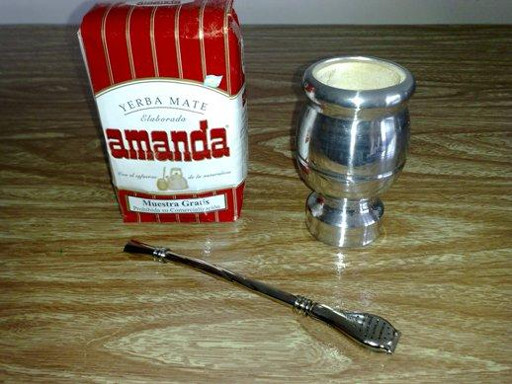
\includegraphics[scale=0.4]{secciones/filtro_color/imagenes/matecocido.jpg}
  
\includegraphics[scale=0.4]{secciones/filtro_color/imagenes/matecocido-fcolor.jpg}
\end{center}
\caption{Imagen antes y después de aplicar el filtro de color con color principal rojo.}
\label{fig:filtro-color-ejemplo}
\end{figure}

La forma en la cual se especifica el rango de colores que deberá permanecer inmutado es mediante la elección de un color principal, cuya codificación RGB se denota con (\param{rc}, \param{gc}, \param{bc}), y un parámetro umbral \param{threshold}. Una vez determinados estos valores, un píxel de la imagen fuente será actualizado por el filtro únicamente si cumple:


\begin{equation} \label{filtro-color-condicion}
\vectornorm{(r, g, b) - (rc, gc, bc)} > threshold 
\end{equation}

donde (\param{r}, \param{g}, \param{b}) es la codificación en RGB del píxel. En particular, de cumplirse esta condición, los tres canales se actualizan de la siguiente forma:

$$ r' = b' = g' = \frac{r + g + b}{3} $$

De esta última expresión se desprende que el color de los píxeles alterados pasa a estar en la escala de grises, ya que los tres canales toman igual valor. Como una observación adicional, queda claro mediante esta especificación que el filtro actúa de forma localizada en sobre cada píxel; su suceptibilidad a ser modificado y su nuevo valor dependen únicamente de su propio valor, y no del de sus vecinos.

\subsection{Implementación en lenguaje C y lenguaje ensamblador}

La implementación en C del filtro se realizó de la forma más sencilla e intuitiva posible; mediante un ciclo que visita una vez a cada píxel de la imagen, de izquierda a derecha y de arriba a abajo, evaluando la condición y modificando su valor de ser necesario. Como única optimización elemental, se modificó la condición (\ref{filtro-color-condicion}) por la siguiente condición equivalente:

$$\vectornorm{(r, g, b) - (rc, gc, bc)}^2 = (r - rc)^2 + (g - gc)^2 + (b - bc)^2 > threshold^2$$

La modificación evita el cálculo de una raíz cuadrada, sin incurrir en el riesgo de exceder el rango del tipo de datos utilizado ya que el máximo \param{threshold} que no hace a la condición trivialmente falsa es $\sqrt{195075} \approx 441$ (el valor máximo que puede tomar la expresión de la izquierda es $255^2 + 255^2 + 255^2 = 195075$), por lo que cualquier valor mayor se puede reducir a $442$.

La implementación en lenguaje ensamblador mantiene esencialmente el mismo procedimiento, con la salvedad de que fue adaptado para procesar cuatro píxeles en simultáneo mediante el uso de operaciones SIMD. Se recorre la matriz en el mismo órden descripto previamente, realizando lecturas de 16 bytes por iteración (equivalente a 5 píxeles y un byte sobrante).

La necesidad de limitar el procesamiento simultáneo a cuatro píxeles se desprende del hecho de que, como se dijo antes, la expresión que mide la distancia entre un píxel y el color principal puede tomar valores en el rango $0, ... \,195075$. Este último valor no cabe en un entero de 16 bits, precisándose un \tipo{double word} para almacenar ese resultado temporal; esto implica un total de hasta cuatro valores de distancia en un registro XMM. En cuestiones de espacio, hubiese sido equivalente utilizar \tipo{floats} ya que también caben hasta cuatro por registro de 128 bits.

De esta forma, el procedimiento realizado en cada iteración consiste en (para cada uno de los cuatro píxeles en simultáneo) comparar el valor de la distancia con el \param{threshold}, y calcular el promedio de los tres canales, actualizando luego sus valores según la siguiente expresión informal:

$$\text{valor\_original} \land \lnot \text{cumple\_condicion} + \text{promedio} \land \text{cumple\_condicion}$$

Esto permite expresar el equivalente a una expresión del tipo \textbf{if}-\textbf{then}-\textbf{else}, en el lenguaje del procesamiento simultáneo.

El cómputo de los flags con el resultado de las comparaciones y del promedio se puede describir mediante el siguiente pseudo-código:

\begin{figure}
	\begin{mdframed}
	\begin{center}
		\begin{lstlisting}
		prom <- [0,0,0,0] 			// enteros doubleword
		dist <- [0,0,0,0]
	
		desempaquetar el rojo de cada pixel a un double word
		rojos <- [r4, r3, r2, r1]
	
		prom += rojos
		rojos -= [rc, rc, rc, rc]
		rojos *= rojos
		dist += rojos
	
		repetir para verdes
		repetir para azules
	
		prom <- prom / 3
		dist <- dist > [threshold, threshold, threshold, threshold]	
		\end{lstlisting}
	\end{center}
	\end{mdframed}
	\caption{Pseudo-código de la implementación en lenguaje ensablador del filtro color.}
\end{figure}

\subsection{Optimizaciones} % (fold)
\label{sub:optimizaciones}



% Describir ocmo funciona el filtro.	
% Como se implementó en c
% Cómo se implementó en asm
	% - explicar el algorítmo
	% - explicar el caso borde
	% - explicar las optimizaciones realizadas. Loop unrolling.
	% - particularidades del filtro. Div 3. Se hicieron todas las cuentas con ints pero al final hubo que pasar a float para poder dividir por 3.
%--Gráfico--  (Performance)
% C vs ASM
% C vs O1, O2, O3
% ASM vs loop unrolling x2 vs loop unrolling 4
% C con y sin condicionales


% Comparar estructura en c y en asm.
	% - En c es un loop que procesa un pixel por vez con un condicional adentro (lo que hace tarde distinta cantidad de tiempo para distintas imágenes).
	% - En asm procesa de a 4 pixeles por vez y hace el mismo proceso independientemente de la imagen.
	% - ¿Que pesa más?¿Procesamiento o acceso a memoria?
	% - Diferencias estructurales
		% - Comparación líneas de código


